 %%%%%%%%%%%%%%%%%%%%%%%%%%%%%%%%%%%%%%%%%% 
 % @File    : c:\Users\Administrator\Desktop\Econometrics\cover\cover.tex
 % @Date    : 2021-02-10 12:15:15
 % @Author  : RankFan
 % @Email   : 1917703489@qq.com
 % -----
 % Last Modified: 2021-02-19 20:58:54
 % Modified By: RankXiaoLong
 % -----
 %%%%%%%%%%%%%%%%%%%%%%%%%%%%%%%%%%%%%%%%%% 

\documentclass[12pt]{article}

\usepackage{ctex}         
\usepackage[left=2cm,right=2cm,top=2.5cm,bottom=3cm]{geometry} % 页面边距
\usepackage{graphicx}%插入图片的宏包。
\usepackage{hyperref}
\hypersetup{ colorlinks,citecolor=blue,linkcolor=blue,urlcolor=red,
			bookmarks, bookmarksnumbered,
			unicode = true }


\begin{document}

\begin{titlepage}
    \centering % Center everything on the title page
    \scshape % Use small caps for all text on the title page
    \vspace*{1.5\baselineskip} % White space at the top of the page
% ===================
%	Title Section 	
% ===================

    \rule{15cm}{1.6pt}\vspace*{-\baselineskip}\vspace*{2pt} % Thick horizontal rule
    \rule{15cm}{0.4pt} % Thin horizontal rule
    
        \vspace{0.75\baselineskip} % Whitespace above the title
% ========== Title ===============	
    {	\Huge 高~等~数~学 ( mathematics )\\ 
            \vspace{4mm}
        课~后~习~题 \\	}
% ======================================
        \vspace{0.75\baselineskip} % Whitespace below the title
    \rule{15cm}{0.4pt}\vspace*{-\baselineskip}\vspace{3.2pt} % Thin horizontal rule
    \rule{15cm}{1.6pt} % Thick horizontal rule
    
        \vspace{1.75\baselineskip} % Whitespace after the title block
% =================
%	Information	
% =================
    {\large 讲课人: \href{http://xiang-tao.github.io/}{向涛} \\
        \vspace*{1.2\baselineskip}
        1689415053@qq.com or xiangtao19970822@gmail.com} \\
        \vspace*{\baselineskip}
    {\large github: \href{https://github.com/Xiang-tao}{Xiang-tao} \\ 
        联系电话:~ 15298155748\\
        \vspace*{\baselineskip}
        
        \vspace*{\baselineskip}
        \today} 
    \vfill

\end{titlepage}
\newpage %开始新的一页
\section{8-3课后习题}
\subsection{习题5}


\includegraphics[scale= 0.6]{8-3-5.png}

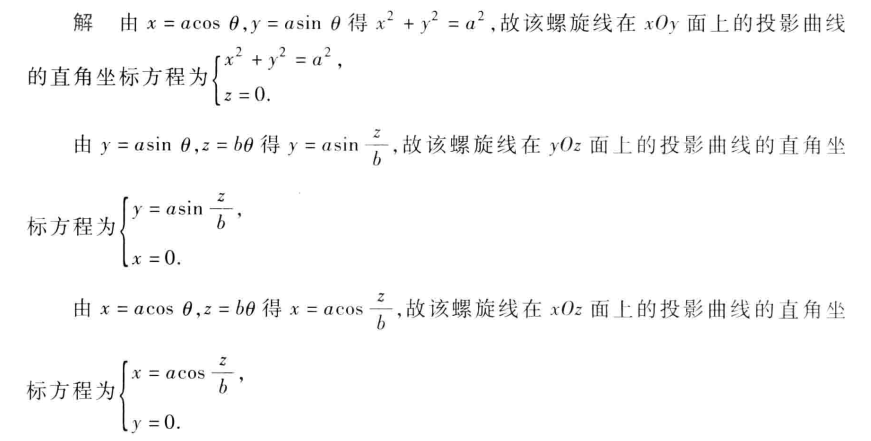
\includegraphics[scale= 0.6]{8-3-5d.png}
%%%%%%%%%%%%%%%%%%%%%%%%%%%%%%%%%%%%%%%%%%%%%%%%%%%%%%%%%%%

\end{document}